\documentclass[10pt, a4paper]{article}
\usepackage[utf8]{inputenc}
\usepackage[T1]{fontenc,url}
\usepackage{multicol}
\usepackage{multirow}
\usepackage{parskip}
\usepackage{lmodern}
\usepackage{microtype}
\usepackage{verbatim}
\usepackage{amsmath, amssymb}
\usepackage{tikz}
\usepackage{physics}
\usepackage{mathtools}
\usepackage{algorithm}
\usepackage{algpseudocode}
\usepackage{listings}
\usepackage{enumerate}
\usepackage{graphicx}
\usepackage{float}
\usepackage{hyperref}
\usepackage{tabularx}
\usepackage{siunitx}
\usepackage{fancyvrb}
%\usepackage{natbib}
%\bibliographystyle{dinat}
\usepackage[makeroom]{cancel}
\usepackage[margin=2.0cm]{geometry}
\usepackage{pdfpages}
\usepackage[margin=10pt, textfont={small, it}, labelfont={bf}, labelsep=endash]{caption}
\renewcommand{\baselinestretch}{1}
\renewcommand{\exp}{e^}
\renewcommand{\b}{\boldsymbol}
\newcommand{\h}{\hat}
\newcommand{\m}{\mathbb}
\newcommand{\half}{\frac{1}{2}}
\renewcommand{\exp}{e^}
\renewcommand{\bar}{\overline}
\setlength\parindent{0pt}


\begin{document}
\title{AST5220\\ Milestone III -- Pertubations}
\author{
    \begin{tabular}{r l}
        Jonas Gahr Sturtzel Lunde & (\texttt{jonassl})
    \end{tabular}}
% \date{}    % if commented out, the date is set to the current date

\maketitle
Code found at \url{https://github.com/asdfbat/AST5220/tree/master/Project}
\vspace{0.7cm}

\section{Introduction}
We have in previous milestones studied the cosmological evolution of the smooth universe, from the relative density functions and their effect on the curvature and conformal time in Milestone I, to the the free electron fraction and its resulting optical depth in Milestone II. In this milestone we introduce perturbations to our smooth universe, which is vital for the observed anisotropies in the cosmic microwave background radiation. This perturbation is naturally included in the Newtonian gauge, which leaves only two degrees of freedom in Einstein equations, namely the two perturbation parameters $\Psi$ and $\Phi$.

The metric perturbations are introduced alongside perturbations in the baryons and CDM, $\delta_{CDM}$ and $\delta_{b}$, as well as perturbations in the photon temperature $\Theta$, and its multipoles $\Theta_\ell$. All the perturbations are solved as a system of ODEs, where the first eight multipoles of the photon temperature are needed for our work in the final milestone. We will analyze the behavior of these perturbations in different density-regimes, as well as before and after horizon entry. Although important components of the CMB creation, neutrinos and polarization will be ignored throughout this milestone.


\section{Theory}
\subsection{Gauge and metric}
In the Newtonian gauge, the metric takes the form of
\begin{equation}
    \begin{aligned}
        g_{00} &= - (1 + 2\Psi(\vec x,t)) \\ 
        g_{ij} &= \delta_{ij}a^2(1 + 2\Phi(\vec x, t))
    \end{aligned}
\end{equation}
with the off-diagonal elements being zero. $\Phi$ and $\Psi$ are known as the Newtonian perturbation parameters, and traces the Newtonian perturbations of the universe.


\subsection{Perturbations and multipoles}
We will be working with perturbations in the energy densities of both baryons and CDM, given as $\delta_{b}$ and $\delta_{CDM}$, as well as the velocity of both, as $v_{b}$ and $v_{CDM}$.

In addition, we need the perturbations in the photon temperature, which we write as
\begin{equation}
    \Theta = \frac{\delta_T}{\bar{T}}
\end{equation}
where $\bar{T}$ and $\delta_{T}$ are the mean temperature and temperature perturbations in the photons, respectively.

In order to calculate the CMB anisotropies, we need the multipole expansions of $\Theta$, defined as\cite{callin2006}
\begin{equation}
\Theta_{l}=\frac{i}{2} \int_{-1}^{1} \mathcal{P}_{l}(\mu) \Theta(\mu) d \mu
\end{equation}
although we will be solving them as a series of coupled ODEs. Although we will solve for the higher order multipoles required calculating the CMB, we will mainly be focusing on $l=0$ and $l=1$ in this milestones results, which defines the photon temperature perturbations and velocities as $\delta_\gamma = 4\Theta_0$ $v_\gamma = -3\Theta_1$.

We will be working in Fourier space, such that all these quantities are functions of wavenumber $(k)$, as well as time $(x)$.


\subsection{System of ODEs}
Having established the quantities of interest as $\delta_{CDM}$, $\delta_{b}$, $v_{CDM}$, $v_{b}$, $\Phi$, $\Psi$, and the chain of multipoles $\Theta_\ell$, we present the coupled ODE system of equations \ref{eqn:ODEstart} - \ref{eqn:ODEstop}. $\Psi$ comes as an explicit expression of $\Phi$, as eqn \ref{eqn:Psi}. Since we are ignoring polarization and neutrinos, we are working with a reduced system of equation. The full system can be found in \cite{callin2006}, and a derivation of most of the equations can be found in \cite{ModernCosmology2003}.

The system of ODEs contains quantities calculated in milestone 1, like the Hubble parameter $\mathcal{H}$, the conformal time $\eta$, and the relative densities $\Omega_r$, $\Omega_{CDM}$, $\Omega_b$, as well as the derivative of the optical depth $\tau'$, from the second milestone.

\begin{align}
    \label{eqn:ODEstart}
    \Theta_{0}^{\prime} &= -\frac{c k}{\mathcal{H}} \Theta_{1}-\Phi^{\prime}\\
    \Theta_{1}^{\prime} &= \frac{c k}{3 \mathcal{H}} \Theta_{0}-\frac{2 c k}{3 \mathcal{H}} \Theta_{2}+\frac{c k}{3 \mathcal{H}} \Psi+\tau^{\prime}\left[\Theta_{1}+\frac{1}{3} v_{b}\right] \\
    \Theta_{\ell}^{\prime} &= \frac{\ell c k}{(2 \ell+1) \mathcal{H}} \Theta_{\ell-1}-\frac{(\ell+1) c k}{(2 \ell+1) \mathcal{H}} \Theta_{\ell+1}+\tau^{\prime}\left[\Theta_{\ell}-\frac{1}{10} \Theta_2 \delta_{\ell, 2}\right], \quad 2 \leq \ell<\ell_{\max } \\
    \Theta_{\ell}^{\prime} &= \frac{c k}{\mathcal{H}} \Theta_{\ell-1}-c \frac{\ell+1}{\mathcal{H} \eta(x)} \Theta_{\ell}+\tau^{\prime} \Theta_{\ell}, \quad \ell=\ell_{\max }
\end{align}


\begin{align}
    \delta_{\mathrm{CDM}}^{\prime} &=\frac{c k}{\mathcal{H}} v_{\mathrm{CDM}}-3 \Phi^{\prime} \\
    v_{\mathrm{CDM}}^{\prime} &=-v_{\mathrm{CDM}}-\frac{c k}{\mathcal{H}} \Psi \\
    \delta_{b}^{\prime} &=\frac{c k}{\mathcal{H}} v_{b}-3 \Phi^{\prime} \\
    v_{b}^{\prime} &=-v_{b}-\frac{c k}{\mathcal{H}} \Psi+\tau^{\prime} R\left(3 \Theta_{1}+v_{b}\right), \quad R = \frac{4\Omega_r}{3\Omega_b a}
\end{align}

\begin{align}
    \label{eqn:ODEstop}
    \Phi^{\prime} &=\Psi-\frac{c^{2} k^{2}}{3 \mathcal{H}^{2}} \Phi+\frac{H_{0}^{2}}{2 \mathcal{H}^{2}}\left[\Omega_{\mathrm{CDM}} a^{-1} \delta_{\mathrm{CDM}}+\Omega_{b} a^{-1} \delta_{b}+4 \Omega_{r} a^{-2} \Theta_{0}\right] \\
    \label{eqn:Psi}
    \Psi &=-\Phi-\frac{12 H_{0}^{2}}{c^{2} k^{2} a^{2}}\left[\Omega_{r} \Theta_{2}\right]
\end{align}

In theory, thousands of multipoles of $\Theta$ are required for accurately calculating the CBM power spectrum. Luckily, thanks to a clever trick called line-of-sight integration, we can limit ourselves to calculating the first eight multipoles, and employ some forbidden magic in the next milestone to generate the rest of the multipoles.


\subsection{Tight coupling regime}
The early universe is in what's called the \textit{tight coupling regime}, meaning that the electrons, photons and baryons are very strongly coupled in a plasma state. In this regime, two effects makes us want to change up the system presented above. Firstly, we don't \textit{need} more than three multipoles of $\Theta$, as the strong coupling means any fluctuation will be very smooth. Secondly, The equations for $v_b$ and $\Theta_1$ are numerically unstable in this regime, due to the extremely high values of $\tau'$, and small values of $\Theta_1$ and $v_b$.

We solve this by replacing the equations for $\Theta_1$ and $v_b$ by
\begin{align}
    q &=\frac{-\left[(1-R) \tau^{\prime}+(1+R) \tau^{\prime \prime}\right]\left(3 \Theta_{1}+v_{b}\right)-\frac{c k}{\mathcal{H}} \Psi+\left(1-\frac{\mathcal{H}^{\prime}}{\mathcal{H}}\right) \frac{c k}{\mathcal{H}}\left(-\Theta_{0}+2 \Theta_{2}\right)-\frac{c k}{\mathcal{H}} \Theta_{0}^{\prime}}{(1+R) \tau^{\prime}+\frac{\mathcal{H}^{\prime}}{\mathcal{H}}-1} \\
    v_{b}^{\prime} &=\frac{1}{1+R}\left[-v_{b}-\frac{c k}{\mathcal{H}} \Psi+R\left(q+\frac{c k}{\mathcal{H}}\left(-\Theta_{0}+2 \Theta_{2}\right)-\frac{c k}{\mathcal{H}} \Psi\right)\right] \\
    \Theta_{1}^{\prime} &=\frac{1}{3}\left(q-v_{b}^{\prime}\right) \\
\end{align}
In addition, $\Theta_2$ now takes the explicit form of
\begin{equation}
    \Theta_2 = - \frac{4ck}{9\mathcal{H}\tau'}\Theta_1
\end{equation}

\subsubsection{Initial conditions}
The intial conditions of our tight coupling system can be found in \cite{callin2006}, and is presented below. The non-tight coupling regime simply takes the initial conditions from the last values in the tight coupling regime.

\begin{align}
    \Psi &=-\frac{2}{3} \\
    \Phi &=-\Psi \\
    \delta_{\mathrm{CDM}} &=\delta_{b}=-\frac{3}{2} \Psi \\
    v_{\mathrm{CDM}} &=v_{b}=-\frac{c k}{2 \mathcal{H}} \Psi \\
    \Theta_{0} &=-\frac{1}{2} \Psi \\
    \Theta_{1} &=+\frac{c k}{6 \mathcal{H}} \Psi \\
    \Theta_2 &= - \frac{4ck}{9\mathcal{H}\tau'}\Theta_1 \\
    \Theta_{\ell} &=-\frac{\ell}{2\ell + 1}\frac{ck}{\mathcal{H}\tau'}\Theta_{\ell - 1}
\end{align}



\section{Implementation}
\subsection{General Overview}
The code used in this report can be found at \url{https://github.com/asdfbat/AST5220/tree/master/Project}. The simulations are found in the \texttt{src/} directory, and is built upon the C++ code template provided by Hans Arnold Winther.

The code builds upon the work from Milestone I \cite{Milestone1} and Milestone II \cite{Milestone2}, and the associated codes, found in \texttt{BackgroundCosmology.cpp} and \texttt{RecombinationHistory.cpp}, respectively.

The code from this milestone is found in the \textit{Perturbations} class, in the \texttt{Perturbations.cpp}, which covers all the coding work done in this milestone. The code, as well as the code from previous milestones, can be compiled and run using the provided \texttt{Makefile}, as \textbf{make all run}. This will write the data files used in the generation of the plots used in this report. The plots are generated by the \texttt{Python/m3\_plotting.ipynb} Jupyter Notebook file.

The end goal of this milestone is to generate splines of all quantities of interest mentioned in the theory section, which will mostly be functions of both $x$ and $k$. The \textit{Perturbations::integrate\_perturbations} method loop over 200 values of $k$, logspaced in $k\in [0.00005,\, 1.0]\, \si{Mpc}$.

\subsection{Solving the ODEs}
For each $k$, a 5000 point array of $x$-values, linearly spaced in $[-16,\, 0]$, is generated for the system to be solver over. The transition point between tight coupling and non-tight coupling is found as the earliest $x$ which fulfills one of the following:
\begin{itemize}
    \item $\qty|\dfrac{k}{\mathcal{H}\tau'}| = \dfrac{1}{10}$
    \item $|\tau'| = 1$
    \item $X_e = 0.99$\quad \text{(Recombination is happening)}
\end{itemize}
Generally, one of these conditions are met around the order of $x \approx -7$

The GSL ODEsolver is employed through a wrapper function in \texttt{ODESolver.cpp} to solve the system of tight coupling ODEs up to the point of the transition.

Upon the end of the tight coupling regime, the last values of the previous solution is inserted as initial conditions for the non-tight coupling solver, which, employing the GSL ODESolver, solves the system of ODEs for the remaining regime.

Once all the solutions are obtained, they are splined using \texttt{Spline.cpp}, a wrapper function for the GSL spline implementation. The splined solutions are written to file, to be plotted.



\section{Results}
\subsection{Newtonian perturbations}
Figure \ref{fig:Phi} shows the evolution of the perturbation parameter $\Phi$ for different modes of k. Since we're ignoring neutrinos and polarization, the other perturbation parameter $\Psi$, turn up to be almost equal to $-\Phi$, as seen in figure \ref{fig:Psi_plus_Phi} in appendix A.

For $\Phi$, we see that for smaller perturbations like $k=0.1Mpc$, there is a quick and sharp fall in $\Phi$ to some value close to zero as it enters the horizon. We know that perturbations undergo a suppression known as the Meszaros effect, if it enters the horizon before the universe has become matter dominated (when the universe becomes non-relativistic). This effect washes out perturbations on the relevant scale at a very high rate, and will as a result suppress the contribution of the relevant scale to the gravitational potential, as we can see from the collapse in $\Phi$.

For larger scales, which enter the horizon later, the effect is reduced. The $k=0.01Mpc$ mode, which enters the horizon just at the transition between radiation and matter domination, the collapse in $\Phi$ is much smaller. At even larger scales, the effect is almost gone altogether, as we can see from the $k=0.001Mpc$ mode.

Towards the end of the plot, we observe an additional collapse in all modes. This is due to the transition to the dark energy dominated era, where perturbations on all scales gets reduced by the high expansion rate of the universe.

\begin{figure}[H]
    \centering
    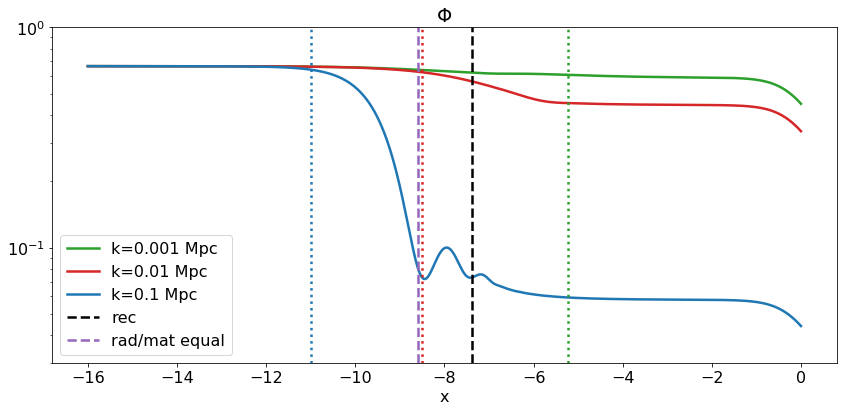
\includegraphics[scale=0.45]{../m3_figs/Phi.png}
    \caption{Figure showing the evolution of $\Psi$ for different k-modes. Horizon entries for each mode is shown as dotted line of corresponding color. Recombination and radiation/matter equality is also shown as striped lines.}
    \label{fig:Phi}
\end{figure}


\subsection{Photon temperature perturbations}
Figure \ref{fig:Thetas} shows the perturbations and velocity in the photon temperature, which we remember are simple functions of the mono- and dipoles, as $\delta_\gamma = 4\Theta_0$ and $v_\gamma = -3\Theta_1$. As each k-mode enters its horizon, we see the perturbation increasing, until it turns, and starts oscillating around some value. For the larger perturbations (smaller k), the oscillations are less prominent, and it settles in at a larger value. The smallest perturbation, at $k=0.1\, Mpc$, settles in around zero.

The velocity shows similar behavior, oscillating around zero for all k-modes, with higher amplitudes for smaller perturbations. We also see a 90 degree phase shift between the perturbations and their velocities, as shown in figure \ref{fig:Thetas_zoomed}. Here we see that the zero-points of the velocities correspond to maxima and minima of the perturbations. As the perturbations grows at its fastest, around its zero-values, we also observe the maxima and minima of the velocities.

\begin{figure}[H]
    \centering
    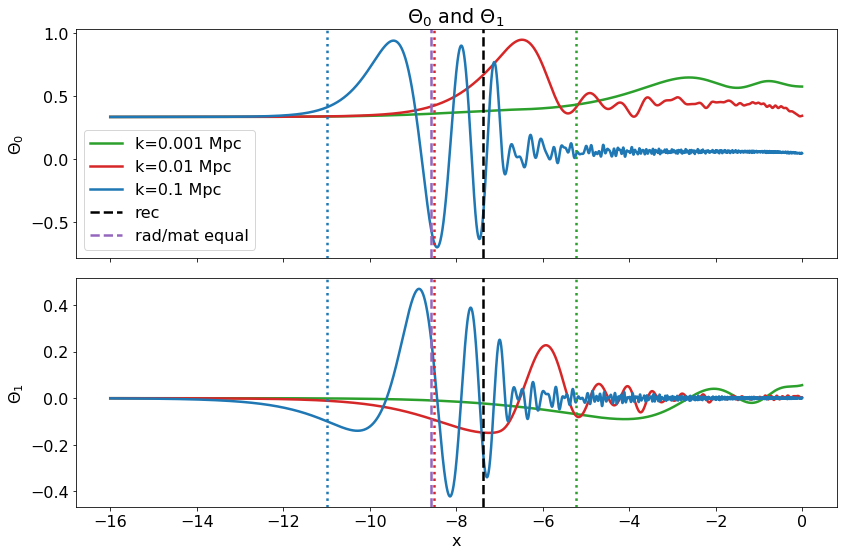
\includegraphics[scale=0.45]{../m3_figs/thetas.png}
    \caption{Figure showing the evolution of the perturbations (top) and velocity (bottom) of the photon temperature for three different k-modes. Horizon entries for each mode is shown as dotted line of corresponding color. Recombination and radiation/matter equality is also shown as striped lines.}
    \label{fig:Thetas}
\end{figure}

\begin{figure}[H]
    \centering
    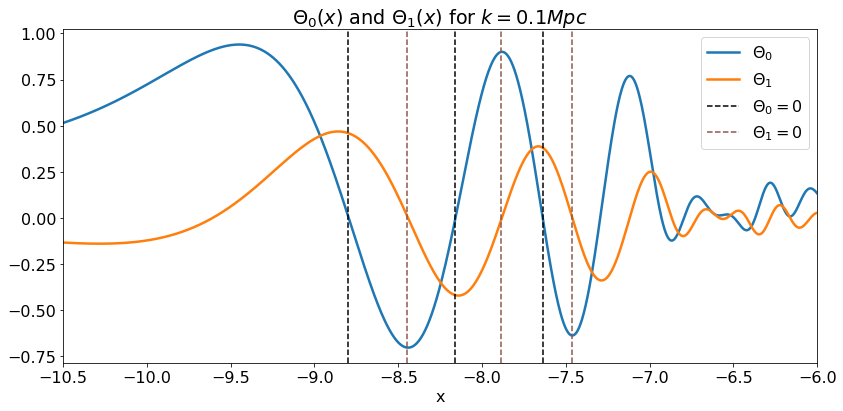
\includegraphics[scale=0.45]{../m3_figs/Theta0_zoomed.png}
    \caption{Monopole and multipole photon temperature perturbations for $k=0.1 Mpc$. The first three zero-points of both functions are indicated as striped lines, and seemingly corresponds with an extremum in the other function, indicating a 90 degrees phase shift.}
    \label{fig:Thetas_zoomed}
\end{figure}


\subsection{Matter perturbations}
Figure \ref{fig:delta_and_v} shows the density perturbations and velocity of the CDM and baryons for the same three k-modes. The CDM for all k-modes have similar trends, where the perturbation starts constant at 1, and starts increasing around horizon entry (dotted line). The baryons trace the CDM exactly for large perturbation, where the horizon entry is in the matter dominated era, and the Meszaros effect is non-existent.

For the smallest perturbation however ($k=0.1\, Mpc$), the baryon perturbation falls off sometime after horizon entry, and starts oscillating around zero. This is due to the pressure-gravity balance, which keeps the baryons from collapsing (until sometime after recombination). The interplay between gravity and pressure makes the baryons expand and contract like an harmonic oscillator. Sometime after recombination, we see the pressure finally giving up, and the baryons collapse into the formed dark matter halos. Without the gravitational wells from dark matter halos, structure growth on this scale would not be possible. For the intermediate k-mode $k=0.01\, Mpc$, we see the baryons slightly fall off the CDM, but quickly catching back up.

For the velocity, we see the same picture as we did for the photon temperature, with a phase transition between the perturbation and its velocity.

Figure \ref{fig:delta_and_v_zoomed} shows a clearer picture of the evolution of a large and a small perturbation, entering the horizon well after and well before matter/radiation equality, respectively. Both start out constantly at a value of one, and the big perturbation transitions to $\propto a$ after it has entered its horizon, which happens well into the matter dominated era. The small perturbation, on the other hand, enters the horizon before matter/radiation equality, and undergoes a transition period known as the Meszaros effect. Here, the growth should run as $\propto \log{a}$. These are, however, analytic approximation, valid deep inside each regime. We see a slope-increase after the horizon-entry, followed by a slope-decrease around $x=-11$, the same point as $\Phi$ reaches its minima for this k-mode.

\begin{figure}[H]
    \centering
    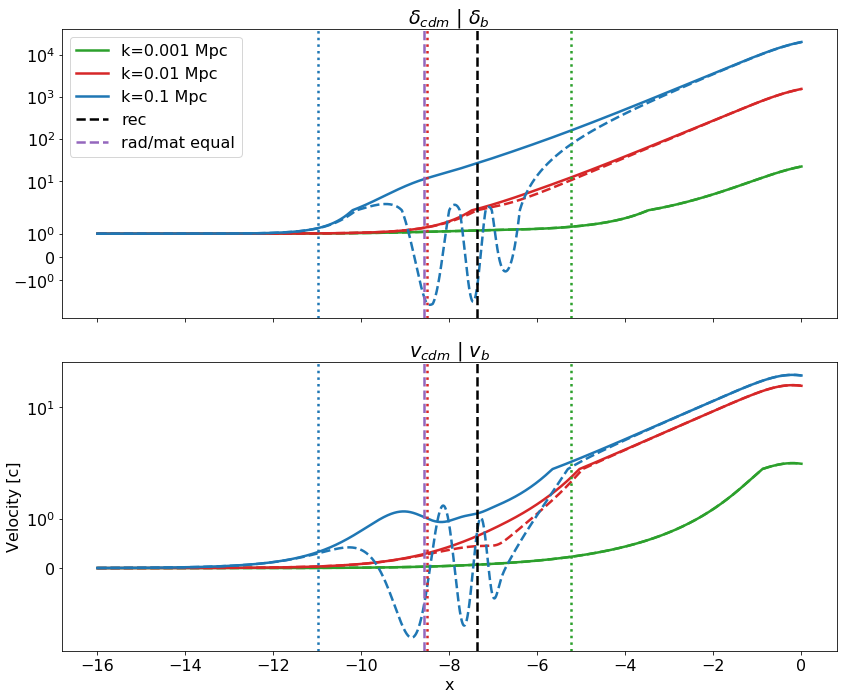
\includegraphics[scale=0.45]{../m3_figs/delta_and_v.png}
    \caption{Figure showing the evolution of the baryon and CDM density perturbations (top) and the baryon and CDM velocity (bottom) for different k-modes. The CDM is shown as continuous lines, while the baryons are shown as striped lines of the same color. Horizon entries for each mode is shown as vertical dotted lines of corresponding color. Recombination and radiation/matter equality is also shown as vertical striped lines.}
    \label{fig:delta_and_v}
\end{figure}

\begin{figure}[H]
    \centering
    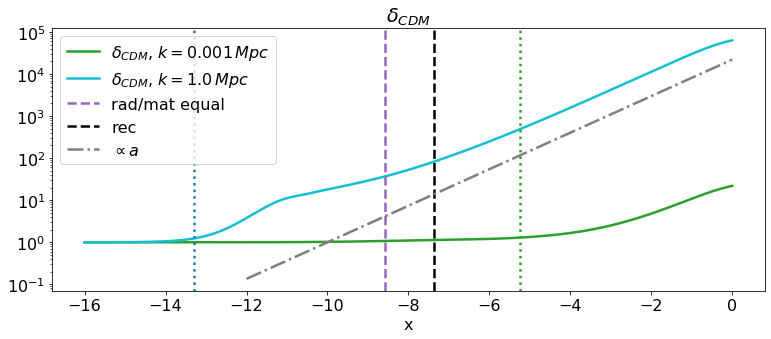
\includegraphics[scale=0.45]{../m3_figs/delta_and_v_zoomed.png}
    \caption{Figure showing the $k=0.1 Mpc$ modes of the density perturbations and velocity of CDM from figure \ref{fig:delta_and_v}. A gray line showing a first power "$a$" proportionality is also shown, for reference.}
    \label{fig:delta_and_v_zoomed}
\end{figure}






\appendix
\section{Phi + Psi}
As we are ignoring polarization and neutrinos, $\Psi$ is nearly equal to $-\Phi$, as we can see from figure \ref{fig:Psi_plus_Phi}.
\begin{figure}[H]
    \centering
    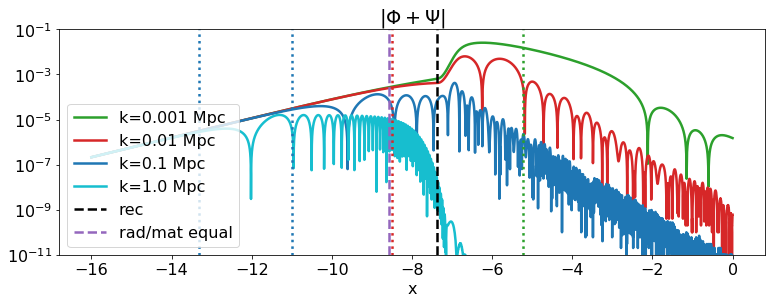
\includegraphics[scale=0.4]{../m3_figs/Psi_plus_Phi.png}
    \caption{Figure showing the absolute sum of $\Phi$ and $\Psi$ for different modes of $k$.}
    \label{fig:Psi_plus_Phi}
\end{figure}






\bibliography{ref}
\bibliographystyle{plain}



\end{document}